\chapter{Metodologia}
\label{cap:4}

Este capítulo apresenta as etapas de desenvolvimento deste trabalho, além de mostrar os códigos propostos e a descrição dos experimentos realizados.

\section{Desenvolvimento do Trabalho}

A metodologia deste trabalho adotou o passo-a-passo exposto na Figura \ref{fig:metodologia}. Inicialmente, foi feita uma pesquisa bibliográfica sobre os temas relacionados a códigos de correção de erros, proteção de TLBs e o efeito da radiação em dispositivos eletrônicos. Realizadas as principais leituras, começamos a desenvolver o código do simulador de TLB, na linguagem de programação Python. O simulador de TLB implementado apresenta as seguintes configurações: cache totalmente associativa, com 8 posições de memória e algoritmo de substituição LRU (do inglês, \textit{least recently used}), além de um NPV com 32 bits.

\begin{figure}[ht]
    \centering
    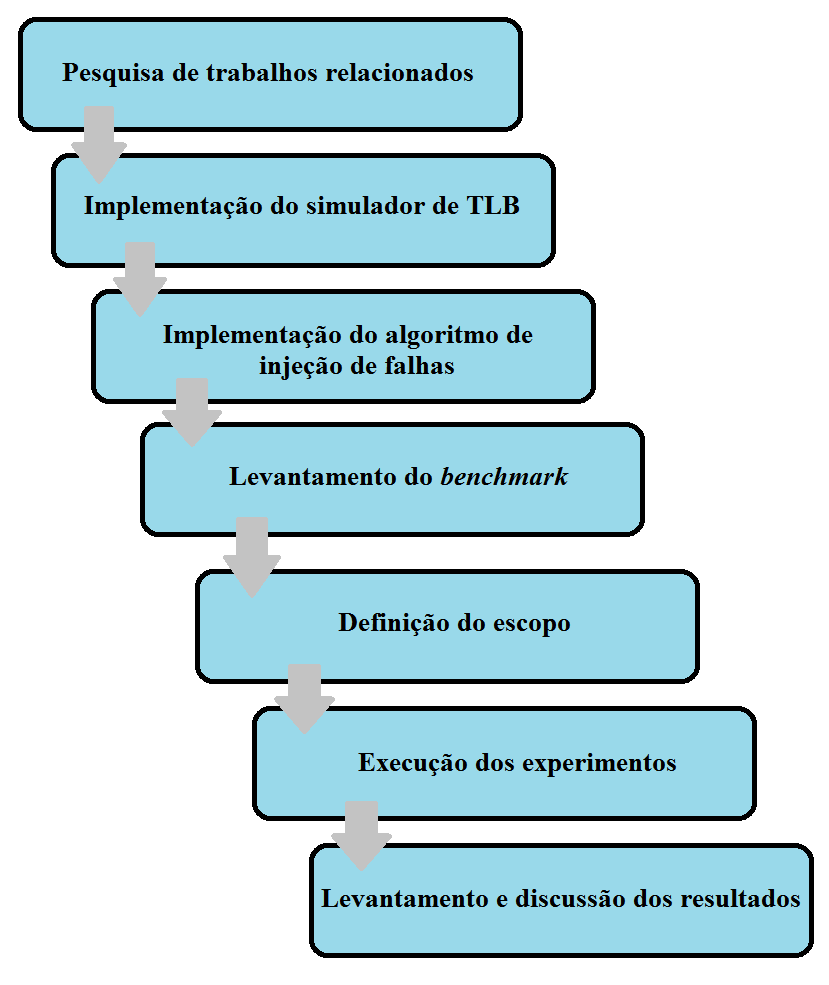
\includegraphics[scale=0.42]{figuras/metodologia.png}
    \caption{Fases do desenvolvimento do trabalho}{Fonte: próprio autor}
    \label{fig:metodologia}
\end{figure}

Em seguida, foi feita a implementação da injeção de falhas. O algoritmo de injeção de falhas desenvolvido é pseudo-aleatório, ocorrendo em posições diferentes a cada nova execução, de acordo com três parâmetros: endereço de falha, que diz em que momento da execução a falha será inserida; linha da tlb, que diz em qual das 8 posições da TLB a falha será injetada; e bit falho, que é referente a qual a posição da falha no NPV, existindo 32 possibilidades de posição. Injetar uma falha em um bit, tendo todos os parâmetros já sorteados, trata-se de alterar o valor desse bit, de 0 para 1 ou vice-versa. Se o tipo de falha é dupla, vai atingir o bit sorteado e o vizinho da direita. Se é falha tripla, atinge os dois vizinhos. A Figura \ref{fig:falhas} apresenta um exemplo para cada um dos três tipos de falha: falha simples (a) atingindo um único bit, falha dupla adjacente atingindo o vizinho da direita (b), e falha tripla adjacente atingindo ambos os vizinhos (c).

\begin{figure}[ht]
    \centering
    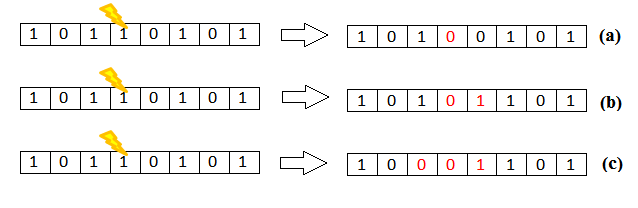
\includegraphics[scale=0.8]{modelo-dissertacao-ppgcc/figuras/falhas.PNG}
    \caption{Exemplos de falha simples (a), falha dupla (b) e falha tripla (c)}{Fonte: próprio autor}
    \label{fig:falhas}
\end{figure}

Após o algoritmo de injeção de falhas, foi feita criação do \textit{benchmark}. O objetivo era encontrar aplicações reais. Após breve pesquisa, foram selecionados códigos com as seguintes aplicações: algoritmo de ordenação (\textit{Merge Sort}), algoritmo de compressão de dados, transformada rápida de Fourier (FFT, do inglês \textit{Fast Fourier Transform}) e filtro digital (Bloom Filter). O \textit{benchmark} com os \textit{traces} de memória utilizados na simulação foi gerado com a ferramenta PIN \cite{luk2005pin}, da Intel.

Em seguida, na etapa de definição do escopo dos experimentos, ficou decidido os cenários a serem testados. Para otimizar a execução, foram consideradas apenas as primeiras 500 mil linhas dos traces de memória gerados pela ferramenta PIN. A simulação foi configurada para executar cada cenário (sem nenhuma proteção, com a codificação proposta por \cite{sanchez2019reducing}, e com os esquemas propostos neste trabalho), com diferentes tipos de injeção de falhas: falhas simples, duplas adjacentes e triplas adjacentes.

Com os experimentos organizados, teve início a execução das simulações. Durante cada execução, o código verifica, assim que a falha é injetada, se o NPV', gerado após sua injeção, é igual a algum NPV já armazenado na TLB. Se não, o valor permanece na memória, até que a palavra com o erro seja substituída ou a simulação acabe. Se houver coincidência, quer dizer que houve indicação de falso positivo, a execução para e contabiliza a ocorrência. Depois de 10 mil execuções para cada cenário, um contador indica qual número de falsos positivos resultou em cada um deles.

A Figura \ref{fig:algoritmo} mostra o algoritmo da simulação. Quando o simulador é executado, o algoritmo verifica o contador em execução. Se o número de execução for <= 10.000, o algoritmo de injeção de falha será executado. Se a simulação executar 10.000 vezes, a simulação termina. A injeção de falha pode causar um falso positivo. No momento em que o simulador encontrar um falso positivo, o simulador para e o contador de falso positivo é incrementado. Se uma falha não for encontrada, o simulador roda até que a palavra com erro injetado seja substituída. Depois que o contador de falsos positivos é incrementado ou a palavra com erro for substituída, o contador de execuções incrementa e o algoritmo reinicia.

\begin{figure}[ht]
    \centering
    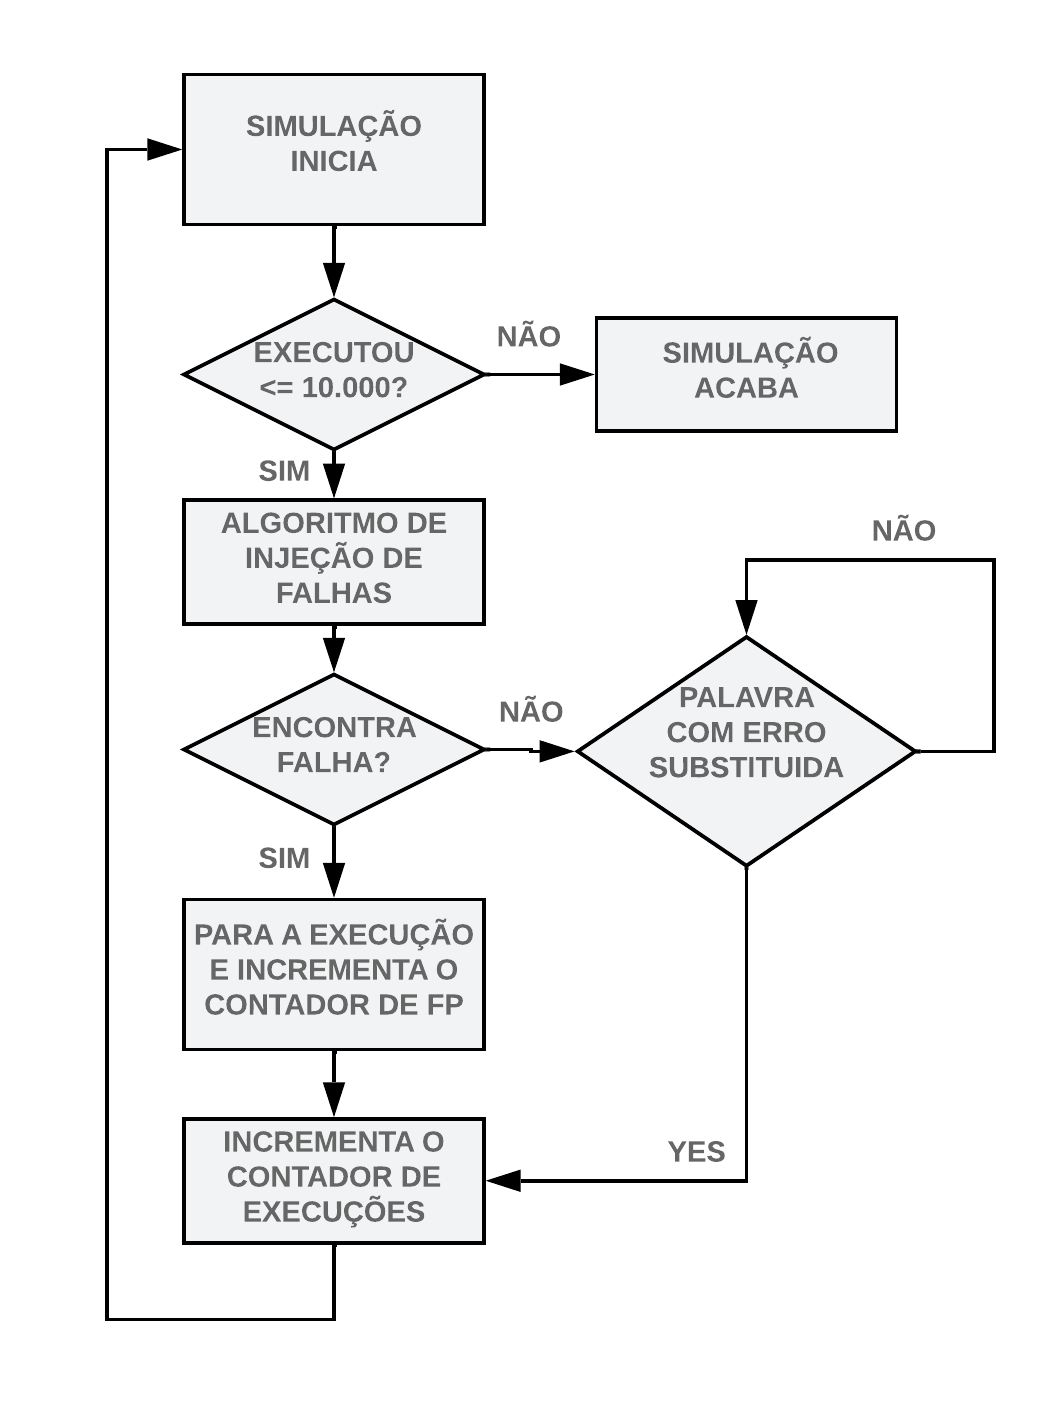
\includegraphics[scale=1]{modelo-dissertacao-ppgcc/figuras/algoritmo.png}
    \caption{Algoritmo da simulação}{Fonte: próprio autor}
    \label{fig:algoritmo}
\end{figure}

Antes de mostrar os resultados obtidos ao final do trabalho, a seção a seguir explica qual a abordagem proposta neste trabalho em adaptação ao código de \cite{sanchez2019reducing}.

\section{Esquema dos códigos propostos}
Este trabalho propõe utilizar uma diferente abordagem da codificação de \cite{sanchez2019reducing}, dessa vez, focando em grupos menores de bits por vez. Isso fica proposto devido ao princípio da localidade espacial, pois em endereços próximos apresenta-se maiores chances de acontecer uma combinação que gere falhas.

Foram propostos quatro cenários: utilizando os 4, 8, 12 e 16 bits mais à direita, ou seja, os menos significativos (LSB, do inglês \textit{least significant bit}), que é justamente onde ocorre a maioria dos falsos positivos.

O objetivo dos métodos propostos é verificar se os códigos seriam capazes de manter a mesma proteção contra falsos positivos que o código que utiliza todos os bits. Deste modo, se comprovado, poderia ter a mesma capacidade de proteção utilizando menos portas XOR, e consequentemente, menos área ocupada na implementação física. 

A Tabela 2 mostra o número de XORs dos cenários propostos em comparação com os do código original, para uma palavra de 32 bits. Como já foi dito anteriormente, a tabela evidencia que são necessárias 30 portas XOR para calcular as duas paridades (MSB e MSB-1) nesse cenário com 32 bits. Para fazer o mesmo com os 16 bits menos significantes, seria preciso 14 portas XOR. É possível notar que o número de portas XOR segue um padrão:
\begin{equation}
    N = B-2
\end{equation}
em que N é o número de portas e B é o número de bits que serão submetidos ao cálculo.

\begin{table}[ht]
\centering
\caption{Número de portas XOR para cada código proposto, comparado com o código original, para um exemplo com 32 bits}
\begin{tabular}{c|c|c|c|c|c}
\hline
\rowcolor[HTML]{EFEFEF} 
\textbf{Código }                            & \textbf{Original} & \textbf{4-LSB} & \textbf{8-LSB} &\textbf{ 12-LSB} & \textbf{16-LSB} \\ \hline
\cellcolor[HTML]{EFEFEF}Portas XOR & 30       & 2     & 6     & 10     & 14     \\ \hline
\cellcolor[HTML]{EFEFEF}\%         & 100      & 6,67  & 20    & 33,33  & 46,67  \\ \hline
\end{tabular}
\end{table}

A Figura \ref{fig:8lsb} exemplifica o circuitos de portas XOR no cenário que calcula os novos valores de MSB e MSB-1 utilizando apenas os 8-LSB, necessitando de 6 portas, reduzindo bastante os custos de implementação do física do código.

\begin{figure}[ht]
    \centering
    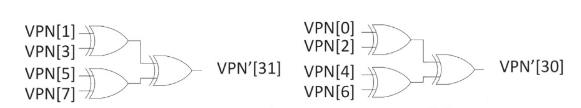
\includegraphics[scale=0.8]{figuras/8lsb.png}
    \caption{Circuito com as portas XOR no cenário de 8-LSB}{Fonte: adaptação de \cite{sanchez2019reducing}}
    \label{fig:8lsb}
\end{figure}

\section{Descrição dos experimentos}

O simulador desenvolvido para este trabalho, conta resumidamente com duas entradas e uma saída. Como mostrado na Figura \ref{fig:metod}, as entradas são os \textit{traces} de memória e o algoritmo de injeção de falhas, enquanto a saída é o número de falsos positivos obtidos naquela simulação. Os \textit{traces} simulam endereços de aplicações reais, que ocuparão as entradas da TLB. Como já foi dito, as aplicações testadas são: \textit{merge sort}, compressão, FFT e \textit{Bloom Filter}. A injeção de falhas insere três tipos de falhas nos bits dos endereços da TLB: erros simples, erros duplos adjacentes e erros triplos adjacentes.

\begin{figure}[ht]
    \centering
    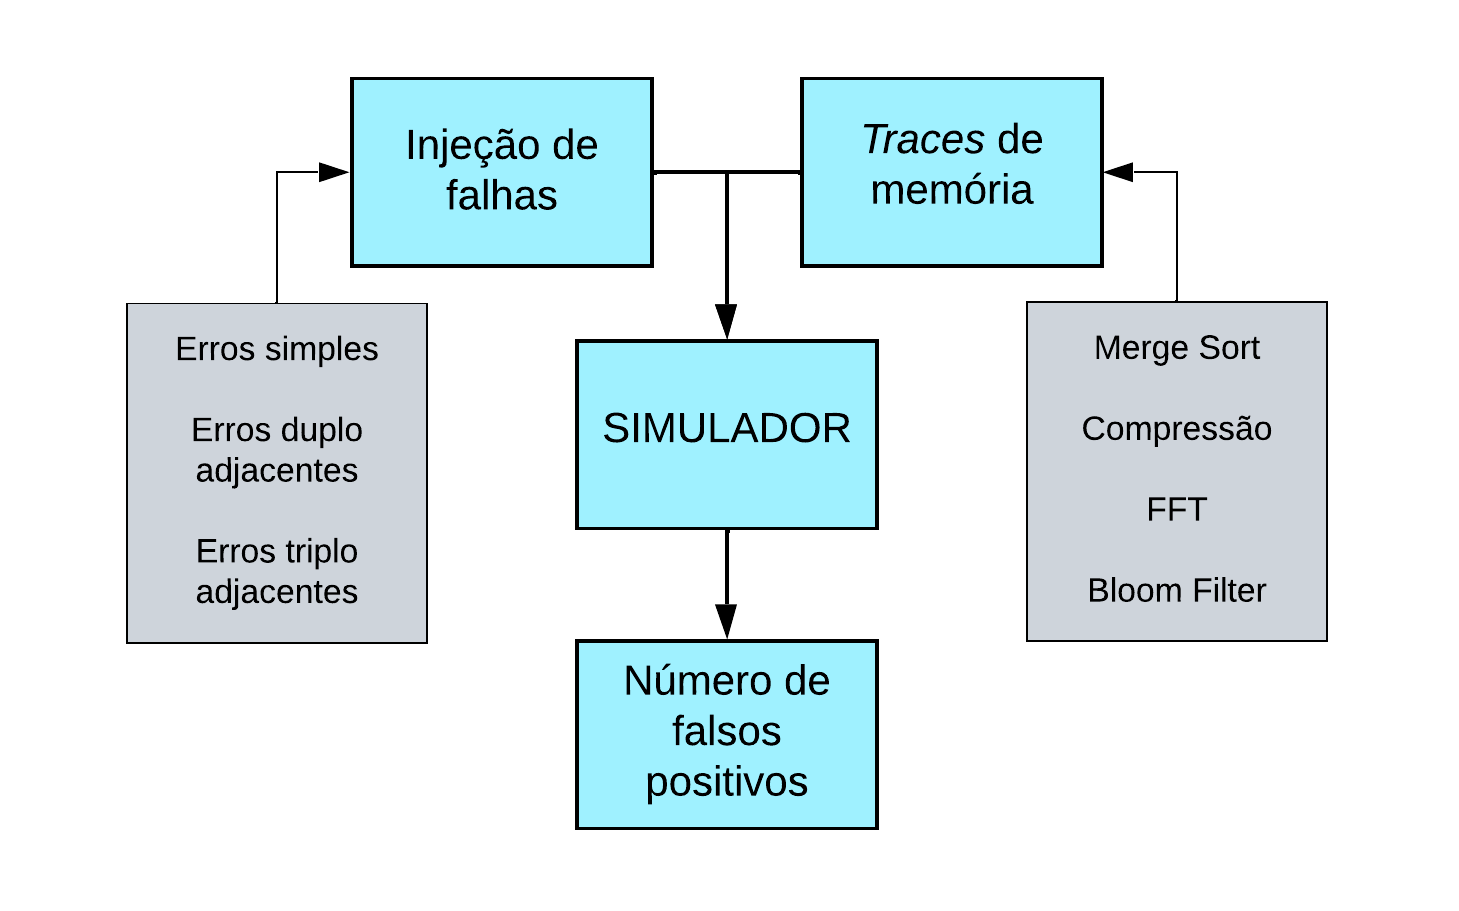
\includegraphics[scale=1]{modelo-dissertacao-ppgcc/figuras/metod.png}
    \caption{Diagrama com entradas e saída do simulador}{Fonte: próprio autor}
    \label{fig:metod}
\end{figure}

Ao fim de cada execução, o simulador retorna 1, para o caso de ter ocorrido falso positivo, ou 0, pro caso de não ter ocorrido. Essa saída é encaminhada para um contador que acumula esse resultado para todas as execuções do mesmo tipo (falha, código e \textit{trace}). 

Após obtidos os números de falsos positivos, esses valores foram convertidos em porcentagem, relacionando o resultado ao número total de execuções para cada cenário, ou seja, 10 mil. Essas porcentagens foram organizadas nas tabelas descritas no Capítulo 4.

\section{Conclusão}

Neste capítulo foi apresentada a metodologia empregada no desenvolvimento do trabalho. Além disso, foram descritos os experimentos realizados, a abordagem dos códigos propostos e as métricas de análise dos resultados. No Capítulo seguintes serão mostrados os resultados desses experimentos.